\chapter{Stato dell'arte}
\label{ch:panoramica}

In questa sezione viene presentata un'analisi comparativa di alcuni dei più famosi sistemi di annotazione esistenti. Lo scopo di questa ricerca è quello di individuare i le caratteristiche comuni ai vari strumenti e le loro limitazioni. Da questa analisi poi è stata stilata una lista di requisiti che portano WATSS ad essere in accordo con gli altri sistemi introducendo allo stesso tempo nuove caratteristiche.

\section{Analisi comparativa di alcuni sistemi di annotazione}

L'analisi dei sistemi si è incentrata principalmente su 3 strumenti open source esistenti: \emph{LabelMe}, \emph{ViPER-GT} e \emph{VATIC}. Per ciascuno dei sistemi è stata stilata una lista di caratteristiche offerte ed evidenziate le eventuali limitazioni. Infine è presentata un'analisi anche con il sistema WATSS.

\subsection{LabelMe}

\emph{LabelMe} è un sistema Web che consente l'annotazione di oggetti all'interno di immagini. Le singole annotazioni sono effettuate mediante la definizione di aree poligonali nell'immagine e l'assegnazione di una label. Il tool offre la possibilità di indicare se un oggetto annotato è occluso o meno da altri oggetti presenti nella scena (non consente però di individuare la parte occlusa o visibile).

Le annotazioni possono essere annidate, è possibile dunque etichettare oggetti che sono inclusi gli uni negli altri. 

In aggiunta alle annotazioni di oggetti il sistema consente di annotare intere aree dell'immagine: questo è reso possibile andando inizialmente a delimitare una porzione di immagine ed associando ad essa una label. In questo caso l'area così definita viene colorata interamente ed è necessario stabilire se si tratta di un'area interna o esterna.

\begin{figure}[H]
\centering
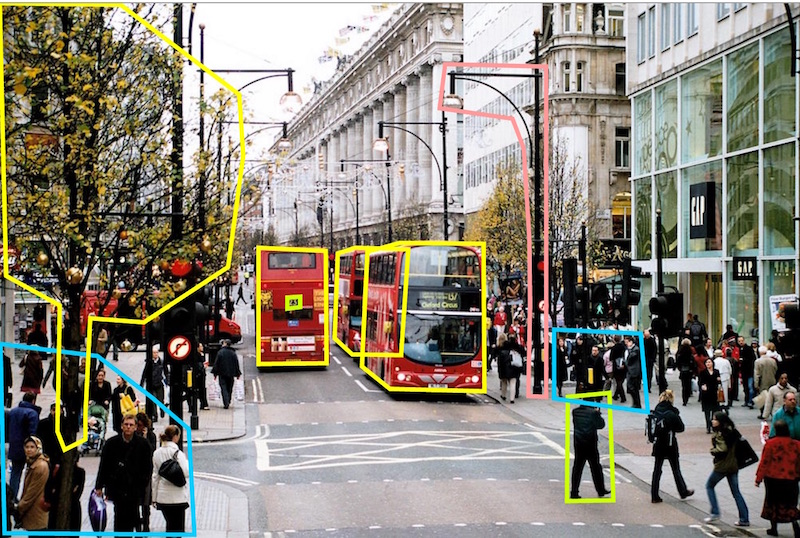
\includegraphics[width=0.6\linewidth]{labelme.jpg}
  \label{fig:labelme}
  \caption{Annotazione di un'immagine tramite LabelMe}
\end{figure}

In fase di esportazione delle annotazioni viene generata una struttura in formato XML che è possibile importare nuovamente in un'altra immagine.

Il sistema non prevede la possibilità di generare \emph{proposals} per le annotazioni, tutto il lavoro è a carico dell'utente.

\subsection{ViPER-GT}

ViPER-GT è un sistema di annotazione per video e la generazione di un \emph{groundtruth}.

ViPER, the Video Performance Evaluation resource, is a set of tools that make video and document algorithm evaluation possible. The two main components, ViPER-Ground Truth and ViPER-Performance Evaluation, provide the ability to mark up videos and documents with ground truth and the ability to compare result data with ground truth, respectively. The extended toolkit, which currently only works on Solaris, provides a more complete solution, with scripting and the ability to generate charts.




is a video annotation tool, a viewer of algorithmically generated markup, a tool for assisting performance evaluation of such markup, and more. This document presents the programs, and details both what it does and does not do. It first contains a tutorial, then a reference, and finally a set of useful information for developers who wish to extend ViPER-GT or use its data format.


\subsection{VATIC}

\subsection{WATSS}
